% !TEX encoding = UTF-8 Unicode
%!TEX root = thesis.tex
% !TEX spellcheck = en-US
%%=========================================
\chapter{Experimental}

\section{Equipment}

\section{Material}

\section{Dataset matching}
\label{sec:method/dataset matching}

Several methods were attempted in order to match the SPED and EDX datasets. The goal was that the matching would be performed automatically with no human input. For this to happen, the code would have to scale, rotate and translate one of the the datasets so that it fit the other. The EDX dataset taken at the intersection of the nanowire and the other elements deposited on it shows a relatively clear separation, and is also the dataset covering the biggest area of the sample. As the SPED dataset was taken over a larger area than the EDX dataset, it was decided to attempt to locate the position of the EDX dataset in the SPED dataset.

%The python library $\mathrm{imreg\_dft}$ \cite{imreg_dft} uses image registration to match two images. Several failed attempts were made using this technique. First, no processing was made to either dataset. The mean was taken in signal space in order to convert them into 2D images, and the intensities were scaled to the range $[0,255]$ so they would be uint8-images. The images were then input into the function, but the result did not come close. Several other attempts were done, following the same structure, except that the datasets were processed in different ways before being converted to 2D images:
%
%\begin{itemize}
%\item Principal component analysis (PCA) was performed on each dataset, and only the component most related to the GaAs nanowire was kept. The nanowire in each of the images now had a high intensity while all other areas were low in intensity.
%\item A similar result was obtained by inserting a virtual annulus in the SPED dataset, so that only a single diffraction spot corresponding to the nanowire was visible. In the EDX dataset, the EDX spectrum was cropped to only include the characteristic peaks corresponding to the nanowire.
%\item A virtual high-angle annular dark field aperture (virtual HAADF) was inserted in the SPED dataset, which was then compared to the DF image taken during the EDX session.
%\item .. background substraction? Thresholding
%\end{itemize}

%As none of these attempts gave any results, another and far more extensive python package, OpenCV \cite{open-cv}, was used instead. The ECC image alignment algorithm \cite{open-cv-ECC} can transform and fit an image using one of three different motions: Translation, euclidian or affine transformation. Here also, different preprocessing steps were taken to make the 2D images of the datasets more similar to each other. The affine transformation uses rotation, translation, scale and shear to fit the images. The euclidian transformation only rotates and translates, so one of the images was rotated before this algorithm was used. The rotation angle was estimated by measuring the angle between the same straight line (the intersection between the nanowire and the deposited elements) in both datasets, and the rotation was performed using the python library sci-kit image \cite{scikit-image}. Finally, the pure translation was attempted, and one of the images was rotated and scaled first. The scaling was performed by selecting the same two points in each datasets, and and using scikit-image to scale by the relative distance between them.
%
%Of these attempts, only the last attempt using the pure translation transformation gave results that were decent, but it was unstable and it was difficult to estimate the accuracy. It also required an unwanted amount of manual input from the user. It was then discovered that the metadata in HyperSpy contained accurate magnification numbers, so these were now used to scale the images relative to each other. It was then attempted to use another OpenCV algorithm, template matching \cite{open-cv-template-matching}, which was described in Section \ref{sec:++++++++}. This algorithm does not detect offset in rotation, so the SPED image was rotated using the manual technique described above.

% Actual solution

The python library OpenCV contains an algorithm which uses template matching, described in \cref{sec:theory/template-matching}, to find the best matching location of one image in another. The algorithm requires that the images are correctly scaled and rotated. To be used with this function, the two datasets first had to be processed to make them look more similar, and to enhance the border of the nanowire. The signal space of each of the datasets was limited to only include signals corresponding to the nanowire. For the SPED dataset, this was done by inserting a virtual annulus that covered only one diffraction spot, which was unique for the nanowire. Similarly, in the EDX dataset, the spectrum was cropped to only include the characteristic $K_\alpha$-peaks of Ga and As. The signal dimension of the datasets were then averaged out, in order to convert them into 2-dimensional arrays, or equivalently, gray-scale images.

The images were now rotated and rescaled. The rotation angle was estimated by selecting two points along the same straight line in both images and finding the angle between them. In the HyperSpy metadata of each of the datasets, a scaling factor giving the size of each pixel was given. The SPED image was rotated through the estimated angle, and the EDX image was rescaled by the ratio between the scaling factors. In order to limit the error caused by manual estimation of the rotational angle, the template matching algorithm was run 100 times for angles in the range $\pm3$\% of the manually estimated angle. In addition, because the contrast levels of the two images are not necessarily equal, the SPED image was multiplied by a gray-scale factor, ranging from 0.80 to 0.85 (this range was found experimentally to give the best results) through 30 steps. For each of the 30 $\times$ 100 iterations of the template matching algorithm, the matching value defined in \cref{eq:matching value} was calculated, and the angle and gray-scale factor giving the lowest matching value were obtained. ++WRITE ABOUT THIRD STEP

After finding the position of the EDX image in the SPED image, the full datasets were processed to enable them to share the same navigation window (define this?). First, the SPED dataset was rotated using T. Aarholt's \textit{rotate}-function \cite{aarholt-rotation}, which is currently awaiting implementation into HyperSpy. Then, the EDX dataset was rescaled and re-binned using K. MacArthur's function \textit{linear\_bin} \cite{kate-binning}, also awaiting implementation into HyperSpy. The functionality of this function is described in \cref{sec:rebin-rotate}. Lastly, a portion of the SPED dataset, corresponding to the location of the EDX image found earlier, was cut out. The two datasets now have the same number of pixels in real space, and each pixel corresponds to the same area of the sample. Using the \textit{Mirror navigation}-function in HyperSpyUI \cite{hyperspyUI}, the two datasets can be made to share a navigation window. 

It then remained to do this for the remaining datasets, all of were are smaller than the dataset used above. Instead of repeating the procedure, the HAADF image, which shows a large area of the sample, was used to find the positions of the remaining datasets with respect to the first. To do this, OpenCV template matching was used to locate the positions of all the datasets in the HAADF image. It was first attempted to use the EDX datasets, converted to images using the technique described earlier. This worked well for the datasets covering a relatively large region of the sample, but not for the smaller ones. Therefore, instead of the datasets, the survey images were used. These images are taken before the EDX recording, and shows a larger region of the sample (is this survey image also HAADF?). After image matching was complete, the matched region was cropped to the actual area of the EDX dataset. The coordinates of this area were found in the survey image's metadata in HyperSpy. 

Lastly, the positions of the remaining datasets had to be found in the SPED dataset. The datasets were again scaled and re-binned to fit the SPED dataset, but now also the coordinates in the HAADF image had to scaled to the SPED dataset, so that the correct area could be cropped out. This step has not been completed.

\section{Quantitative analysis}

\begin{figure}
	\centering
	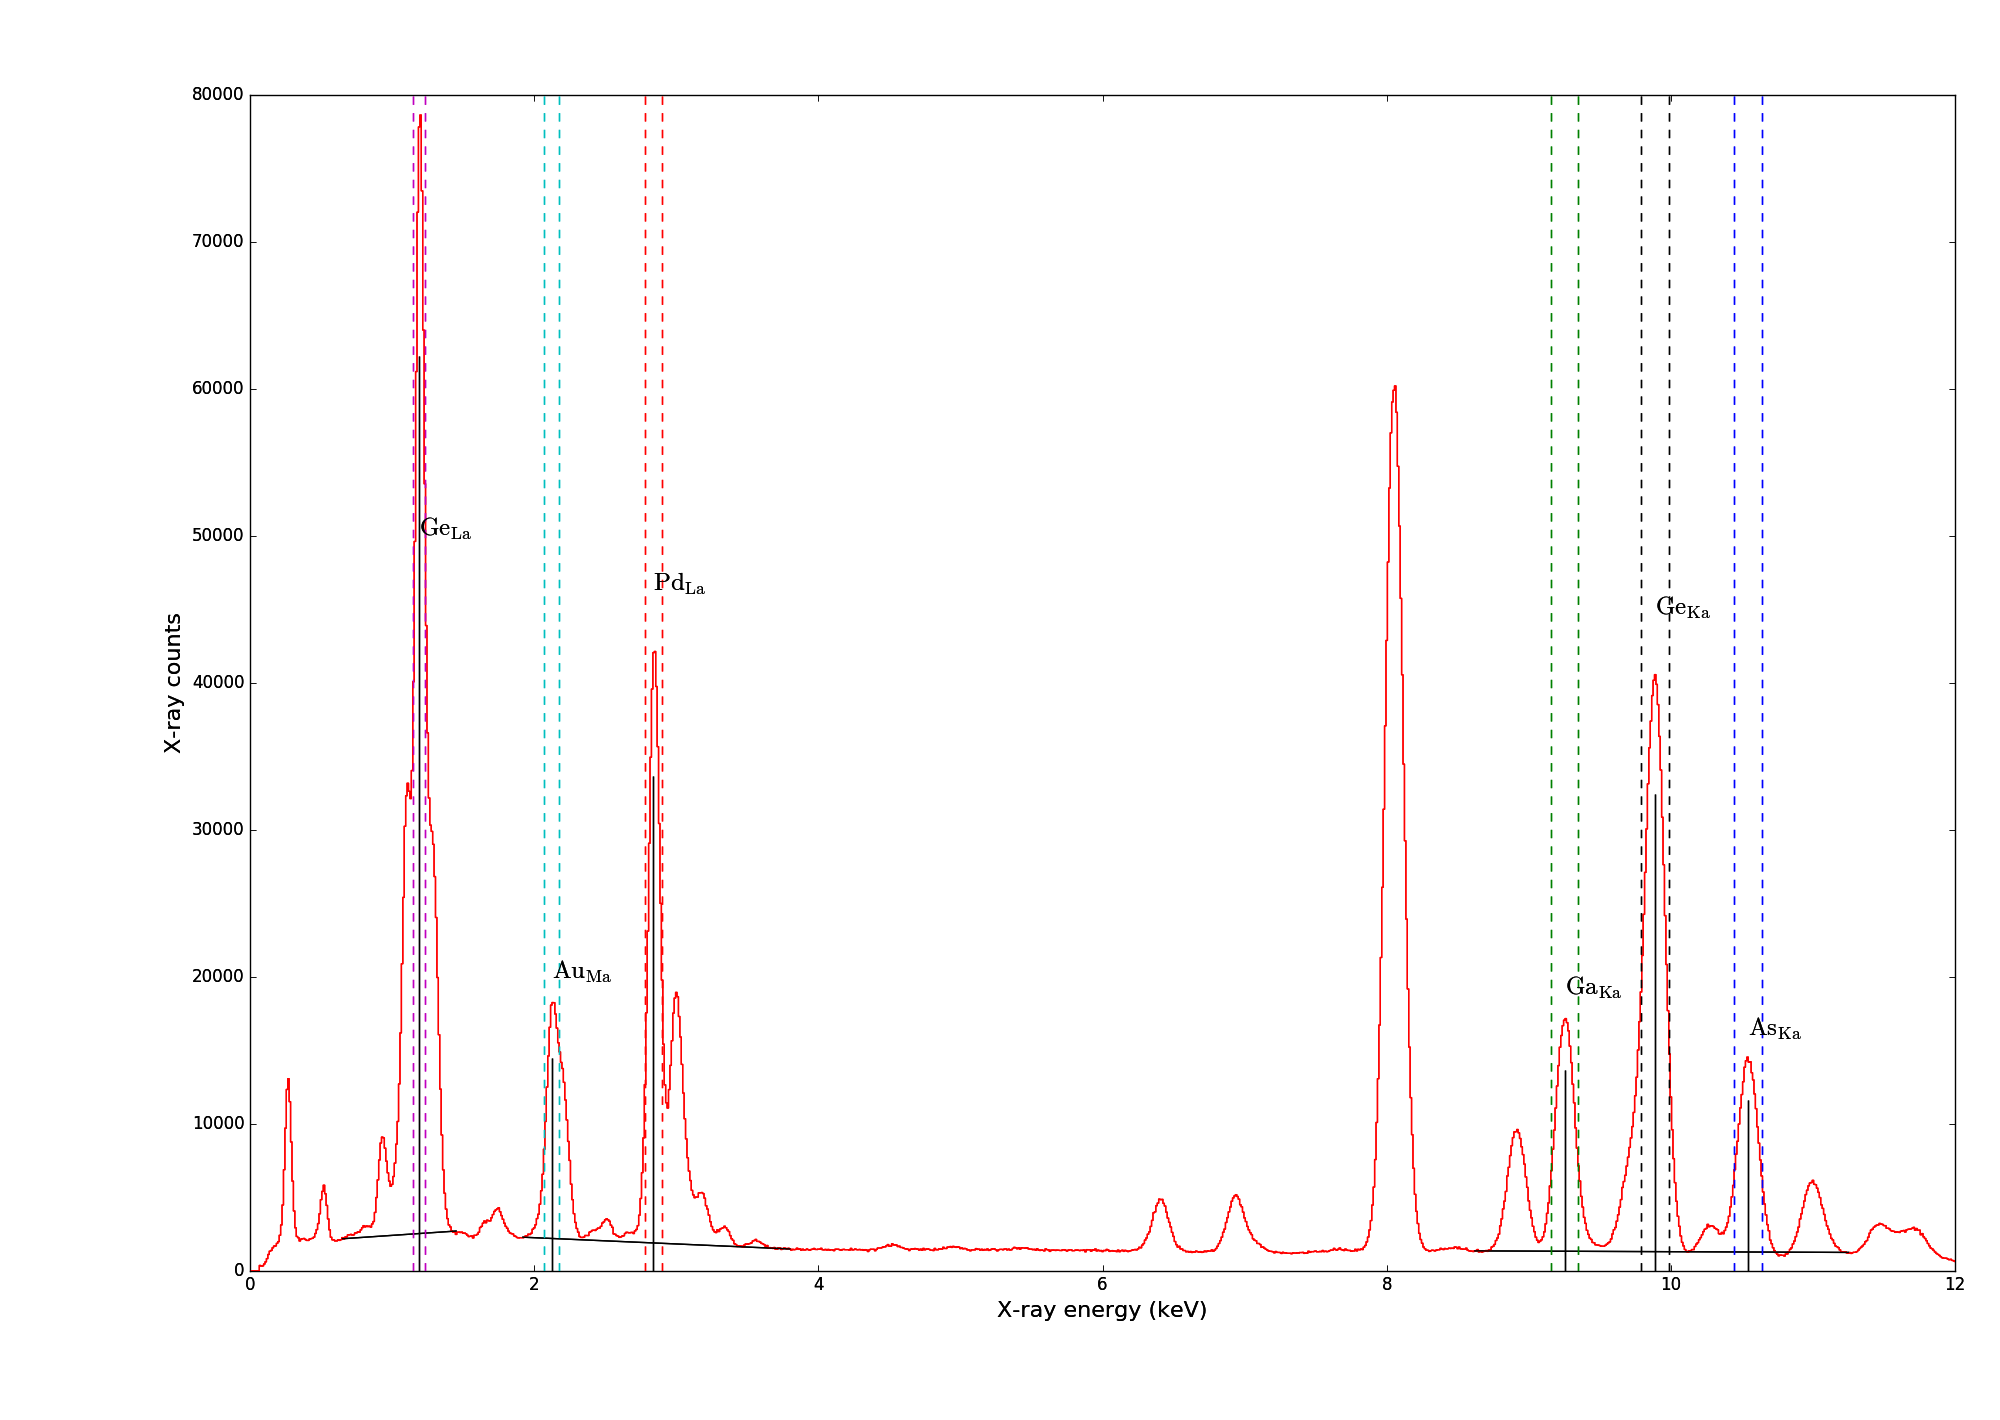
\includegraphics[width=0.7\linewidth]{fig/other/UnheatedA-full-spectrum2}
	\caption{}
	\label{fig:spectrum-with-info}
\end{figure}
The first step in the quantitative analysis was to determine the $\zeta$-factors of the elements in the sample. As this method had not yet been implemented into HyperSpy \cite{hyperspy}, the necessary code was acquired from the Master's thesis of A. Garmannslund \cite{andreas}. The thickness of the material was estimated using a thickness map (see Section ????). Background subtraction was performed by selecting an area of the background signal at both sides of each characteristic line, and drawing a line between the centers of these two areas. The intensities of the lines were then calculated by integrating over the peaks within an integration window of 1.2 FWHM. \cref{fig:spectrum-with-info} shows the characteristic X-ray peaks that have been used, the background that has been subtracted and the integration windows.

Thickness map

The quantification of the samples was performed using three different methods: The Cliff-Lorimer ratio technique, for which the necessary $k$-factors were obtained from the TEM software, the $\zeta$-factor method and the $\zeta$-factor method with background subtraction. HyperSpy was used for the first two of these methods, but absorption correction is at the time not been included in the software. The necessary code for this was also acquired from Garmannslund's thesis. All three techniques were used, in order to enable the results to be compared against each other. To verify the techniques, they were first used on the untreated sample whose composition is assumed to be known. They were then used on the heated sample in order to determine the composition at locations of interest.